\documentclass{article}
 

\usepackage{amsmath}
\usepackage{amssymb}
\usepackage{graphicx}
\usepackage{verbatim}
\usepackage{enumerate}
\usepackage{epstopdf}
\usepackage{epsfig}

\newcommand{\beq}{\begin{equation}}
\newcommand{\eeq}{\end{equation}}

\begin{document}
\title{Project 4. FYS3150}
\author{Shafa Aria}
\maketitle
\newpage
\section{Introduction: Diffusion of neurotransmitters in the synaptic cleft}

In the following project we will turn our attention to the transportation of signals between neurons (nerve cells) in the brain. 
The dominant way of transporting these signals is by means of diffusion of particular signal molecules called \textit{neurotransmitters}.
\begin{figure}[thb]
\centerline{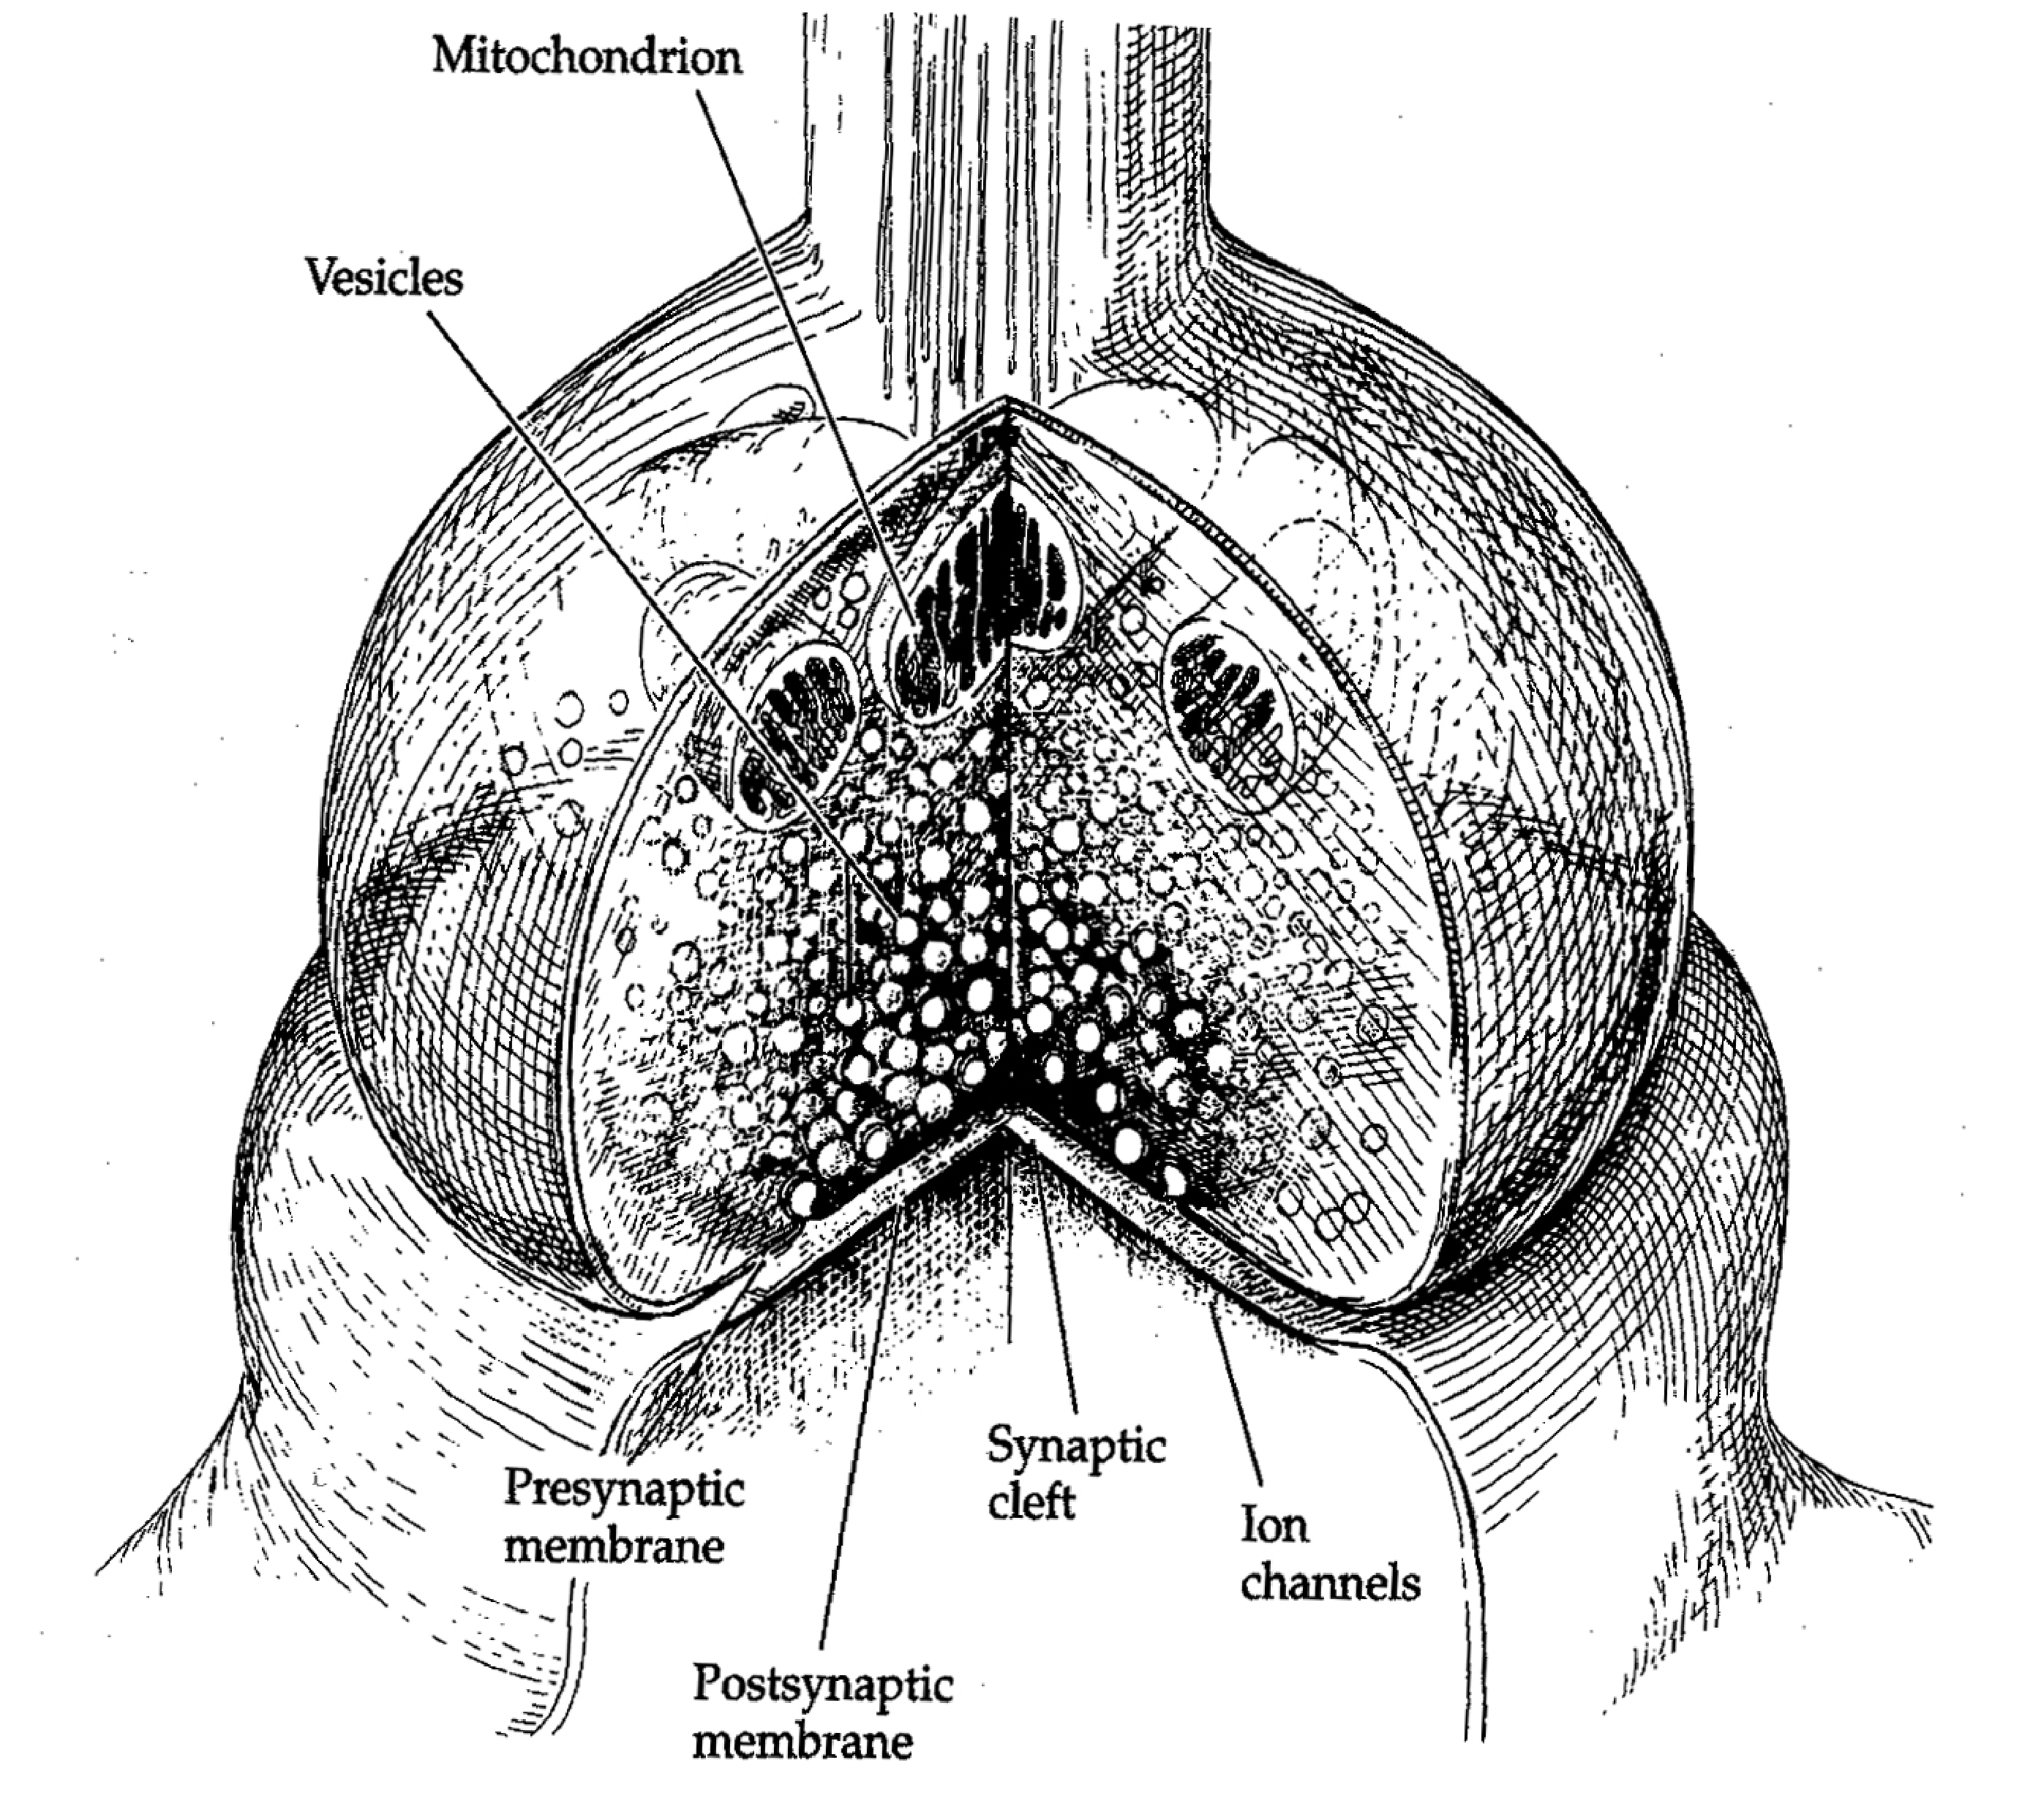
\includegraphics[width=9cm]{thompsonB2000-p38.eps}}
\caption{\small Drawing of a synapse. The axon terminal is the knoblike
structure and the spine of the receiving neuron is the bottom one. The
synaptic cleft is the small space between the presynaptic (axon)
and postsynaptic (dendritic spine) membrane.
(From Thompson: ``The Brain'', Worth Publ., 2000)}
\label{fig:figure1}
\end{figure}

Fig.~\ref{fig:figure1} depicts how the signals are being transported across the synaptic cleft. \\
\begin{figure}[t]
\centerline{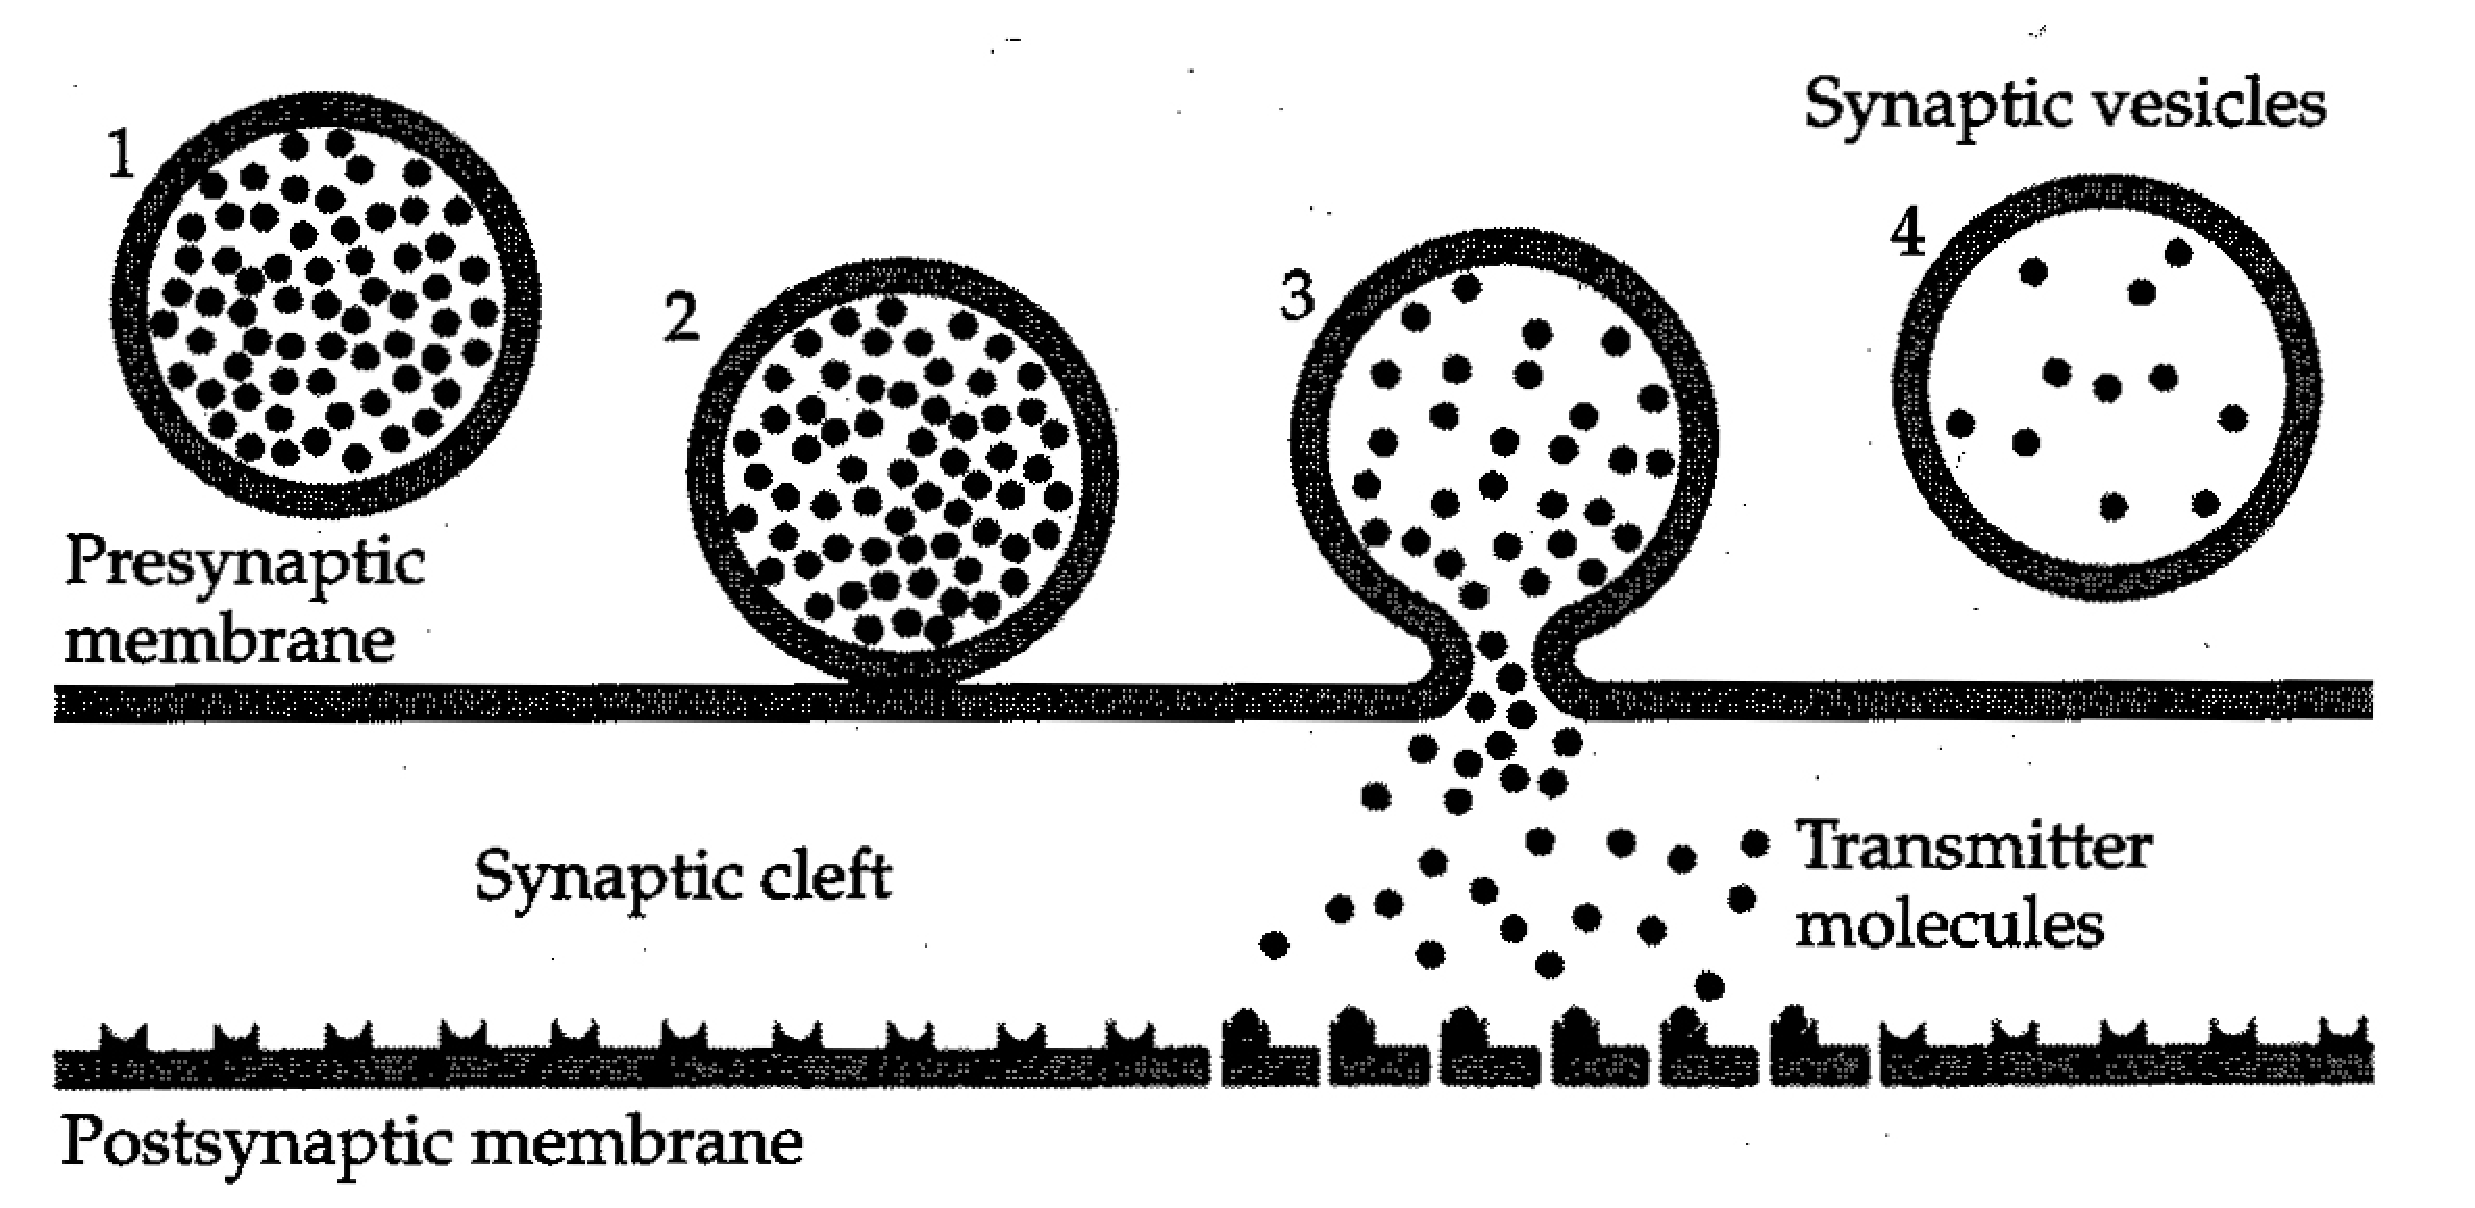
\includegraphics[width=10cm]{thompsonB2000-p39.eps}
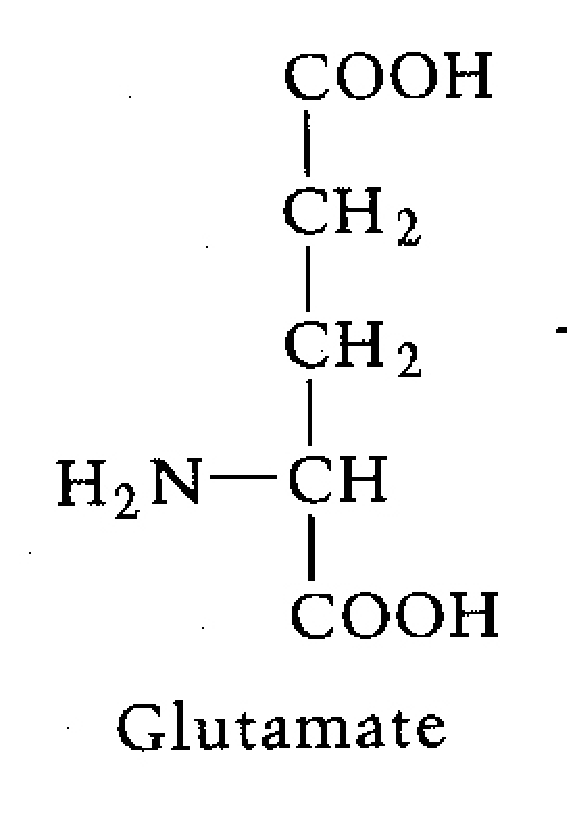
\includegraphics[width=3cm]{kandel-B1991-p217-glutamate.eps}
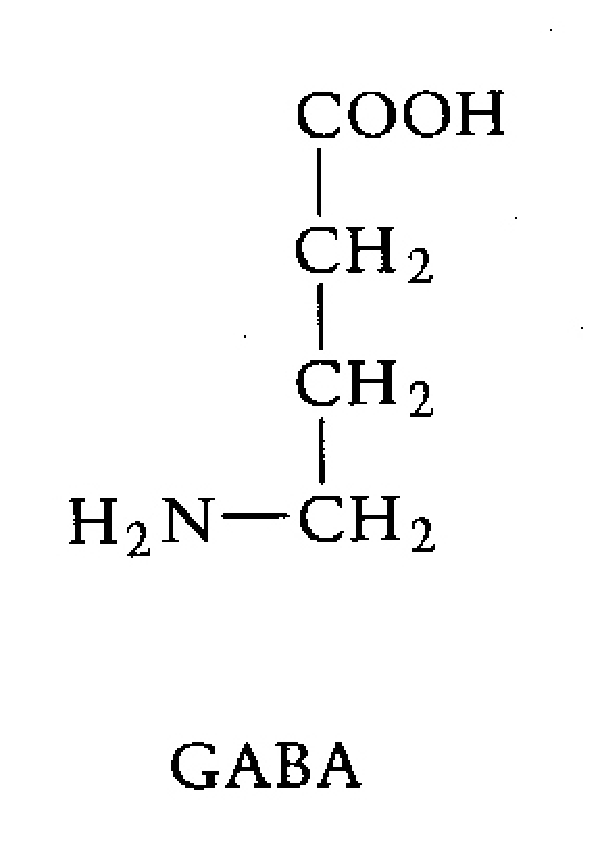
\includegraphics[width=3cm]{kandel-B1991-p217-GABA.eps}}
\caption{\small Left: Schematic drawing
of the process of vesicle release from the axon terminal and release of
transmitter molecules into the synaptic cleft. (From Thompson: ``The
Brain'', Worth Publ., 2000). Right: Molecular structure of the
two important neurotransmitters \emph{glutamate} and \emph{GABA}.}
\label{fig:figure2}
\end{figure}
Following the arrival of an action potential in the axon terminal a
process is initiated in which (i) vesicles inside the axon terminal
(filled with neurotransmitter molecules) merge with the presynaptic
(axon) membrane and (ii) release neurotransmitters into the synaptic
cleft. These neurotransmitters diffuse across the synaptic cleft to
receptors on the postsynaptic side which ``receives'' the signal.
A schematic illustration of this process is shown in
Fig.~\ref{fig:figure2}(left).

Since the transport process in the synaptic cleft is governed by
diffusion, we can describe it mathematically by
%
\begin{equation}
\frac{\partial u}{\partial t} = D \nabla^2 u,
\label{eq:diffusion_eq_3D}
\end{equation}

where $u\,$ is the concentration of the particular neurotransmitter, and
$D$ is the diffusion coefficient of the neurotransmitter in this
particular environment (solvent in synaptic cleft).

If we assume (i) that the neurotransmitter is released
roughly equally on the ``presynaptic'' side of the synaptic cleft, and
(ii) that the synaptic cleft is roughly equally wide across the whole
synaptic terminal, we can, given the large area of the synaptic cleft
compared to its width, assume that the neurotransmitter concentration
only varies in the direction across the synaptic cleft (from
presynaptic to postsynaptic side). We choose this direction to be the
$x$-direction (see Fig.~\ref{fig:figure3}).

In this case $u({\bf r})=u(x)$, the diffusion equation
reduces to
%
\begin{equation}
\frac{\partial u}{\partial t} = D \frac{\partial^2 u}{\partial x^2}.
\label{eq:diffusion_eq_1D}
\end{equation}\newline
Immediately after the release of a neurotransmitter into the
synaptic cleft ($t=0$) the concentration profile in the $x$-direction
is given by
%
\begin{equation}
u(x,t=0) = N \, \delta(x),
\label{eq:initial_condition}
\end{equation}
%
where $N$ is the number of particle released into the synaptic cleft
per area of membrane.
To get an idea over the time-dependence of the neurotransmitter
concentration at the postsynaptic side ($x=d$), we can look at the
solution of a ``free'' random walk (i.e., no obstacles or particle
absorbers in either direction). The
solution of Eq.~(\ref{eq:diffusion_eq_1D}) with the initial condition
in Eq.~(\ref{eq:initial_condition}) is given by 
(see Nelson: \emph{Biological Physics}, p. 143 or Lectures notes chapter 12.3)
%
\begin{equation}
u(x,t) = \frac{N}{\sqrt{4 \pi D t}} e^{-x^2/4Dt}\;\;.
\label{eq:solution_delta_1D}
\end{equation}\newline
The concentration at the postsynaptic side $u(d,t)$
approaches 0 in the limit $t \rightarrow 0\;$ and
$t \rightarrow \infty$. 

The above assumption regarding the
neurotransmitter molecules undergoing a ``free'' random walk, is
obviously a simplification. In the true diffusion process in the
synaptic cleft the neurotransmitter molecules will, for example,
occasionally bump into the presynaptic membrane they came from. Also
at the postsynaptic side the neurotransmitters are absorbed by
receptors located on the postsynaptic cell membrane and are thus
(temporally) removed from the solution.

To approach this situation in our mathematical model we can impose the
following boundary and initial conditions with $x\in[0,d]$
%
\begin{equation}
u(x=0,t>0) = u_0, \;\;u(x=d,\mbox{all $t$})=0,
\;\;u(0 < x < d,t < 0) = 0 \;\;.
\label{eq:initial_conditions_2}
\end{equation}
Hereafter we set $d=1$.
This corresponds to that (i) for $t<0$ there are no neurotransmitters
in the synaptic cleft, (ii) for $t>0$ the concentration of
neurotransmitters at the presynaptic boundary of the synaptic
cleft ($x=0$) is kept
\emph{fixed}  at $u=u_0=1$ in our case, and (iii) that the postsynaptic receptors
immediately absorb nearby neurotransmitters so that $u=0$ on the
postsynaptic side of the cleft ($x=d=1$).


The full solution of the diffusion equation with
boundary/initial conditions in Eq.~(\ref{eq:initial_conditions_2})
can be found in a closed form. We will use this solution to test our numerical calculations.
%
%%%%%%%%%%%%%%%%%%%%%%%%%%%%%%%%%%%%%%%%%%%%%%%%%%%%%%%%%%%%%
%
% FIGURE : synaptic cleft
\begin{figure}[b]
\centerline{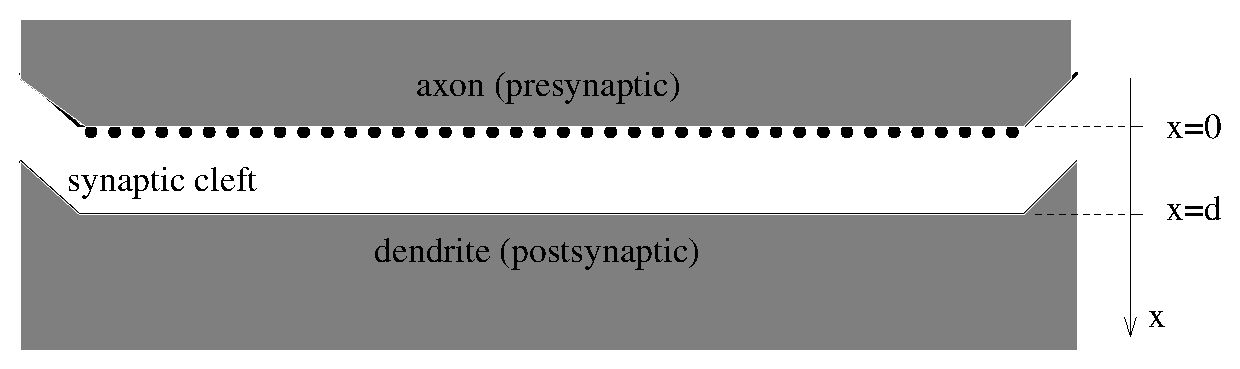
\includegraphics[width=10cm]{synaptic_cleft.eps}}
\caption{\small Schematic drawing of the synaptic cleft in our model. The
black dots represent neurotransmitter molecules, and the situation
shown corresponds to the situation immediately after neurotransmitter
release into the synaptic cleft.}
\label{fig:figure3}
\end{figure}
%
%%%%%%%%%%%%%%%%%%%%%%%%%%%%%%%%%%%%%%%%%%%%%%%%%%%%%%%%%%%%%
%

We are thus looking at a one-dimensional
problem 
\[
 \frac{\partial^2 u(x,t)}{\partial x^2} =\frac{\partial u(x,t)}{\partial t}, t> 0, x\in [0,d]
\]
or 
\[
u_{xx} = u_t,
\]
with initial conditions, i.e., the conditions at $t=0$, 
\[
u(x,0)= 0 \hspace{0.5cm} 0 < x < d
\]
with $d=1$ the length of the $x$-region of interest. The 
boundary conditions are 
\[
u(0,t)= 1 \hspace{0.5cm} t > 0,
\]
and 
\[
u(d,t)= 0 \hspace{0.5cm} t > 0.
\]
In this project we want to study the numerical stability of three methods for partial differential equations
(PDEs). 
These methods are 
\begin{enumerate}
\item The explicit forward Euler algorithm with discretized versions of time given by a forward formula and
a centered difference in space resulting in
 \[
u_t\approx \frac{u(x,t+\Delta t)-u(x,t)}{\Delta t}=\frac{u(x_i,t_j+\Delta t)-u(x_i,t_j)}{\Delta t}
\]
and
\[
u_{xx}\approx \frac{u(x+\Delta x,t)-2u(x,t)+u(x-\Delta x,t)}{\Delta x^2},
\]
or
\[
u_{xx}\approx \frac{u(x_i+\Delta x,t_j)-2u(x_i,t_j)+u(x_i-\Delta x,t_j)}{\Delta x^2}.
\]
\item The implicit Backward Euler with
 \[
u_t\approx \frac{u(x,t)-u(x,t-\Delta t)}{\Delta t}=\frac{u(x_i,t_j)-u(x_i,t_j-\Delta t)}{\Delta t}
\]
and
\[
u_{xx}\approx \frac{u(x+\Delta x,t)-2u(x,t)+u(x-\Delta x,t)}{\Delta x^2},
\]
or
\[
u_{xx}\approx \frac{u(x_i+\Delta x,t_j)-2u(x_i,t_j)+u(x_i-\Delta x,t_j)}{\Delta x^2},
\]
\item Finally we use the implicit Crank-Nicolson scheme with 
a time-centered scheme at $(x,t+\Delta t/2)$
 \[
u_t\approx \frac{u(x,t+\Delta t)-u(x,t)}{\Delta t}=\frac{u(x_i,t_j+\Delta t)-u(x_i,t_j)}{\Delta t}.
\]
The corresponding spatial second-order derivative reads
\[
u_{xx}\approx \frac{1}{2}\left(\frac{u(x_i+\Delta x,t_j)-2u(x_i,t_j)+u(x_i-\Delta x,t_j)}{\Delta x^2}+\right.
\]
\[
\left. \frac{u(x_i+\Delta x,t_j+\Delta t)-2u(x_i,t_j+\Delta t)+u(x_i-\Delta x,t_j+\Delta t)}{\Delta x^2}
\right).
\] 
Note well that we are using a time-centered scheme wih $t+\Delta t/2$ as center.
\end{enumerate}
%%%%%%%%%%%%%%%%%%%%%%%%%%%%%%%%----------Solving the project starts here------------- %%%%%%%%%%%%%%%%%%%%%%%%%%%
\section{Solving the diffuse equation}
We are now going to head on finding a closed form solution for our equation
$$\frac{\partial^2 u(x,t)}{\partial x^2} = \frac{\partial u(x,t)}{\partial t}, x \in [0,d]$$
With the initial conditions and boundary conditions we gave above. One of the reasons we wish to find the closed solution is to estimate the numerical accuracy of our results obtained by the numerical methods. 
In order to carry out this, we will need to find the steady-state solution which is on the form $u(x) = Ax + b$, which 
we can easily verify by setting the RHS of the above PDE to zero and using $$y(x) = c_1e^{r_1x} + c_2xe^{r_1x}$$ where $r_1 = 0$. 
Which indeed gives us: $$u_s(x) = c_1 + c_2x$$
with the boundary conditions applied, with $u(0) = 1$:
$$1 = c_1$$
and $u(d=1) = 0$:
$$c_2 = -1$$
Which gives us: $$u_s(x) = 1 - x$$
Now we will head over finding $u(x)$ and combining the two solutions we can derive $v(x) = u(x) - u_s(x)$ with boundary conditions
$v(0) = v(d) = 0$. This will make solving the equation both numerically and on closed form easier because of the more friendlier boundary conditions.
\subsection{Finding $u(x)$}
We start by noting down once again the initial and boundary conditions:
\beq
u(x,0) = 0, \hspace{2cm} u(0,t) = 1, \hspace{2cm} u(d,t) = 0 \nonumber
\eeq
Before we embark on an endless journey to solve $u(x,t)$ it would be much wiser to induce the above equation to derive new boundary conditions:
$$v(x,t) = u(x,t) - u_s(x)$$
Getting new initial and boundary conditions:
\begin{align*}
v(x,0) &= u(x,0) - u_s(x) = 1 - x\\
v(0,t) &= u(0,t) - u_s(0) = 1 - 1 = 0\\
v(d,t) &= u(d,t) - u_s(d) = 0 - (1-1) = 0\\
\end{align*} 
Where we in the last one used the fact that $d=1$. 
our new boundary and initial conditions are thereby $v(x,0) = x-1$, $v(0,t) = 0$ and $v(d,t) = 0$.

Then we note that our PDE is one dimensional and only depends on $x$ and $t$, hence we can try solving it by separation of variables:
$$v(x,t) = X(x)T(t)$$ 
which we insert into our PDE and get:
\begin{align*}
T(t)\frac{\partial^2 X(x)}{\partial x^2} & = X(x) \frac{\partial T(t)}{\partial t}\\
\frac{1}{X(x)}\frac{\partial^2 X(x)}{\partial x^2} & = \frac{1}{T(t)} \frac{\partial T(t)}{\partial t}
\end{align*} 
Now we want that the equations to hold for all $x$ and $t$ and hence require that the RHS and LHS to be equal to a constant which we will call $-\lambda^2$. 
\beq
\frac{1}{X(x)}\frac{\text{d}^2 X(x)}{\text{d} x^2}  = -\lambda^2, \hspace{2cm} \frac{1}{T(t)} \frac{\text{d} T(t)}{\text{d} t} = -\lambda^2 \nonumber
\eeq
\beq
\frac{\text{d}^2 X(x)}{\text{d} x^2}  + \lambda^2X(x) = 0, \hspace{2cm} \frac{\text{d} T(t)}{\text{d} t} + \lambda^2T(t) = 0 \nonumber
\eeq
The root of our solution has the form $z = \lambda i$ for the spatial component which is complex and hence we have:
$$X(x) = A\sin(\lambda x) + B\cos(\lambda x)$$
For the time component:
\begin{align*}
\frac{\text{d}T}{\text{d} t} &= -\lambda^2 T \\
\ln(T) &= -\lambda^2t
\end{align*}
Which gives us:
\beq
X(x) = A\sin(\lambda x) + B\cos(\lambda x), \hspace{2cm} T(t) =  Ce^{-\lambda^2t}
\eeq
Following our boundary conditions we get $B=0$, and since we are looking for non-trivial solutions:
\beq
0 = A\sin(\lambda d) \nonumber
\eeq 
which results in $\lambda d = n\pi \rightarrow \lambda_n = \frac{n\pi}{d}$ for $n = 1,2,3...$
We now see that we can have infinitely many eigenvalues and hence also eigenfunctions for the spatial part. Setting together the spatial and the time part:
$$v(x,t) = A_n\sin(\frac{nx\pi}{d})e^{-\frac{n^2\pi^2t}{d^2}}$$
for $n=1,2,3...$\\
Now we know from the principles of superposition that if we have two linear homogeneous differential equations, then their sums will also be a solution.
Thereby our solution becomes:
\beq
v(x,t) = \sum_{n=1}^\infty A_n\sin(\frac{nx\pi}{d})e^{-\frac{n^2\pi^2t}{d^2}}
\eeq
This, again will satisfy any initial condition in the form:
$$v(x,0) = u_s(x) = \sum_{n=1}^\infty A_n\sin(\frac{nx\pi}{d})$$
And we realise that this is indeed the Fourier sine series and we can then determine $A_n$ from the theorem of Fourier series:
$$A_n = \frac{2}{d} \int_0^d u_s(x)\sin(\frac{nx\pi}{d})\text{d}x$$
Where $u_s(x) = x-1$ and for $n=1,2,3...$
Solving the integral gives us: $$A_n = -\frac{2}{n\pi}$$
%----------We introduce the algos-----
\section{The algorithms}
For this project we are going to determine the stability and accuracy of the three following algorithms.
\subsection{Explicit Scheme}
For the Explicit Scheme we start off with out usual $u_{xx} = u_t$ equation that we need to solve. 
Which is nothing else that the diffusion equation with two boundary conditions and one initial condition.
To arrive at the algorithm we introduce step lengths to both the space variable $x$ and the time $t$, with $$\Delta x=\frac{1}{n+1}$$
and a $\Delta t$ for the time. The position after $i$ steps and the time at the time-step $j$ are given by
$$t_j = j\Delta t \hspace{1cm} j>0$$
$$x_i = i\Delta x\hspace{1cm} 0\le i\le n+1$$

We then use the standard approximation for the derivative and the second derivative to obrain solutions for the time and spatial part:
\begin{align*}
u_t \approx \frac{u(x_i, t_j + \Delta t) - u(x_i, t_j)}{\Delta t}\\
u_{xx} \approx \frac{u(x_i + \Delta x, t_j) - 2u(x_i, t_j) + u(x_i - \Delta x, t_j)}{\Delta x^2}
\end{align*} 
We have a local error of $O(\Delta x^2)$. We can simplify these even further with our notation:
$$u_t \approx \frac{u_{i,j+1} - u_{i,j}}{\Delta t}$$
$$u_{xx} \approx \frac{u_{i+1,j} - 2u_{i,j} + u_{i-1,j}}{\Delta x^2}$$
Now if we set these two equations equal to each other and solve for $u_{i,j+1}$ we get:
$$u_{i,j+1} = \alpha u_{i-1,j} + (1 -2\alpha)u_{i,j} + \alpha u_{i+1,j}$$
Where $\alpha = \Delta t/\Delta x^2$.
The stability condition for our explicit scheme is $\Delta t/\Delta x^2 \le 1/2$. During programming we omit the $\Delta t$ altogether and just stick to $\alpha$.

\subsection{Implicit Scheme}
Same as above only this time we use the backward formula for the derivative:
$$u_t \approx \frac{u(x_i, t_j) - u(x_i, t_j -\Delta t)}{\Delta t}$$
With our spatial part as before. Again setting the equations equal and solving this time for the implicit $u_{i,j-1}$:
$$u_{i,j-1} = -\alpha u_{i-1,j} + (1 -2\alpha)u_{i,j} - \alpha u_{i+1,j}$$
This leads us to tridiagonal matrix on the form:
$$\hat{A} = \begin{bmatrix}
       1+2\alpha &  -\alpha  & 0           & 0        & \cdots  \\[0.3em]
       -\alpha   & 1+2\alpha & -\alpha 	   & 0        & \cdots  \\[0.3em]
       \vdots 	 & \vdots    & \vdots      & \vdots   & \cdots  \\[0.3em]
       \vdots    & \vdots    & \vdots      & \vdots   & \cdots  \\[0.3em]
       \vdots    & \vdots    & \vdots      & \vdots   & -\alpha \\[0.3em]
       0         & 0         & \cdots      & -\alpha  & 1+2\alpha
     \end{bmatrix} $$

And hence we can treat the problem as a vector-matrix multiplication:
$$\hat{A}V_j = V_{j-1}$$
Where our $$V_j = \begin{bmatrix}
					u_{1,j} \\
					u_{2,j} \\
					\vdots  \\
					u_{n,j} 
				\end{bmatrix}$$

Since we are dealing with a tridiagonal matrix it is much more useful computational wise to use methods for solving the tridiagonal matrices as this will decrease the operations needed from $~O(N^3)$ to $~O(N)$.

\subsection{Crank-Nicolson Scheme}
For this scheme we are going to combine the implicit and explicit to create a new scheme. We introduce a new parameter $\theta$ adding the two schemes from before and adding the new parameter we have:
$$\frac{\theta}{\Delta x^2}(u_{i-1,j} - 2u_{i,j} +u_{i+1,j}) + \frac{1-\theta}{\Delta x^2}(u_{i+1,j-1} - 2u_{i,j-1} + u_{i-1,j-1}) = \frac{1}{\Delta t}(u_{i,j} - u_{i,j-1})$$
If $\theta = 0$ we get the forward formula and hence the explicit scheme and if $\theta = 1$ we get the backward formula and hence the implicit scheme. For $\theta = 1/2$ we get the Crank-Nicoloson scheme.
This can be rewritten on the form:
$$ -\alpha u_{i-1,j} + (2 +2\alpha)u_{i,j} - \alpha u_{i+1,j}= \alpha u_{i-1,j-1} + (2 -2\alpha)u_{i,j-1} + \alpha u_{i+1,j-1}$$
or once again in vector form:
$$(2\hat{I} + \alpha\hat{B})V_j = (2\hat{I} - \alpha\hat{B})V_{j-1}$$
Where we already have defined the previous matrices and where 
$$\hat{B} = \begin{bmatrix}
       2         & -1        & 0           & 0        & \cdots  \\[0.3em]
       -1        & 2         & -1 	       & 0        & \cdots  \\[0.3em]
       \vdots 	 & \vdots    & \vdots      & \vdots   & \cdots  \\[0.3em]
       \vdots    & \vdots    & \vdots      & \vdots   & \cdots  \\[0.3em]
       \vdots    & \vdots    & \vdots      & \vdots   & -1 \\[0.3em]
       0         & 0         & \cdots      & -1       & 2
     \end{bmatrix} $$
This scheme has a truncation in time which goes $O(\Delta t^2)$ and is, like the implicit scheme, stable for all possible combinations of $\Delta t$ and $\Delta x$
\section{References}

\end{document}